\section{Prediction Performance of HDP}
\label{sec:Result}
In this section, we present the experimental results of the HDP approach to address RQ1.

{\bf RQ1: Is heterogeneous defect prediction comparable to WPDP, existing CPDP approaches for heterogeneous metric sets (CPDP-CM and CPDP-IFS), and UDP?}

RQ1 leads us to investigate whether our
HDP is comparable to WPDP (Baseline1), CPDP-CM
(Baseline2), CDDP-IFS (Baseline3), and UDP (Baseline4). We report the representative HDP results in Section~\ref{subsec01},~\ref{subsec02},~\ref{subsec03}, and~\ref{subsec04-0} based on Gain ratio attribute selection for metric selection, KSAnalyzer with the cutoff threshold of 0.05, and the Logistic classifier.
Among different metric selections, Gain ratio attribute selection with Logistic led to the best prediction performance overall. In terms of analyzers, KSAnalyzer led to the best prediction performance.
Since the KSAnalyzer is based on the p-value of a statistical test, we chose a cutoff of 0.05 which is one of commonly accepted significance levels in the statistical test~\cite{Corder09}.

In Section~\ref{subsec04},~\ref{subsec05}, and~\ref{subsec06}, we report the HDP results by using various metric selection approaches, metric matching analyzers, and machine learners respectively to investigate HDP performances more in terms of RQ1.

%----------------------------------------------------------
\subsection{Comparison Result with Baselines}
\label{subsec01}% KSAnalyzer with the cutoff of %
% 0.05}
%----------------------------------------------------------

\begin{table*}[!t]
%\footnotesize
%\small
%\scriptsize
\centering
\caption{Comparison results among WPDP, CPDP-CM, CPDP-IFS,
and HDP by KSAnalyzer with the cutoff of 0.05 in a median AUC. (Cliff's $\delta$ magnitude --- N: Negligible, S: Small, M: Medium, and L: Large)
%  Outperforming results with statistical
%  significance (Wilcoxon signed-rank test, p$<$0.05) between within and cross by
%  the proposed approach and between cross using common features and those by the
%  proposed approach are bold-faced and underlined respectively.
}
\label{tab:result_overview}
%\setlength{\tabcolsep}{5pt}
%\setlength{\extrarowheight}{1.5pt}
%\begin{tabular}{|@{ }c@{ }||@{}c@{}|@{}c@{}|@{}c@{}||@{}c@{}|}
%\begin{tabular}{|@{}c@{}||@{}c@{}||@{}C{21mm}@{}|@{}C{21mm}@{}|@{}C{21mm}@{}||@{}C{8mm}@{}|}
\begin{tabular}{|c||c|c|c|c||c|}
\hline
{\bf Target}
& \specialcell{{\bf WPDP}\\{(Baseline1)}}
&\specialcell{{\bf CPDP-CM}\\{(Baseline2)}}
&\specialcell{{\bf CPDP-IFS}\\{(Baseline3)}}
&\specialcell{{\bf UDP}\\{(Baseline4)}}
&\specialcell{{\bf HDP}\\{\bf KS}}%\\{cutoff=0.05}}
\\
\hline \hline
EQ  &{\bf 0.801} (-0.519,L) &0.776 (-0.126,{\bf N}) &0.461 (0.996,{\bf L})  &0.737 (0.312,{\bf S})  &0.776* \\ \hline
    JDT &{\bf 0.817} (-0.889,L) &0.781 (0.153,{\bf S})  &0.543 (0.999,{\bf L})  &0.733 (0.469,{\bf M})  &0.767* \\ \hline
    LC  &{\bf 0.765} (-0.915,L) &0.636 (0.059,{\bf N})  &0.584 (0.198,{\bf S})  &0.732$^{\&}$ (-0.886,L)        &0.655 \\ \hline
    ML  &{\bf 0.719} (-0.470,M) &0.651 (0.642,{\bf L})  &0.557 (0.999,{\bf L})  &0.630 (0.971,{\bf L})  &0.692*$^{\&}$ \\ \hline
    PDE &{\bf 0.731} (-0.673,L) &0.681 (0.064,{\bf N})  &0.566 (0.836,{\bf L})  &0.646 (0.494,{\bf L})  &0.692* \\ \hline
    Apache      &{\bf 0.757} (-0.398,M) &0.697 (0.228,{\bf S})  &0.618 (0.566,{\bf L})  &0.754$^{\&}$ (-0.404,M)        &0.720* \\ \hline
    Safe        &0.829 (-0.002,{\bf N}) &0.749 (0.409,{\bf M})  &0.630 (0.704,{\bf L})  &0.773 (0.333,{\bf M})  &\underline{0.837}*$^{\&}$ \\ \hline
    ZXing       &0.626 (0.409,{\bf M})  &0.618 (0.481,{\bf L})  &0.556 (0.616,{\bf L})  &0.644 (0.099,{\bf N})  &{\bf 0.650} \\ \hline
    ant-1.3     &0.800 (-0.211,S)       &0.781 (0.163,{\bf S})  &0.528 (0.579,{\bf L})  &0.775 (-0.069,{\bf N}) &0.800* \\ \hline
    arc &0.726 (-0.288,S)       &0.626 (0.523,{\bf L})  &0.547 (0.954,{\bf L})  &0.615 (0.677,{\bf L})  &0.701 \\ \hline
    camel-1.0   &0.722 (-0.300,S)       &0.590 (0.324,{\bf S})  &0.500 (0.515,{\bf L})  &0.658 (-0.040,{\bf N}) &0.639 \\ \hline
    poi-1.5     &0.717 (-0.261,S)       &0.675 (0.230,{\bf S})  &0.640 (0.509,{\bf L})  &0.720 (-0.307,S)       &0.706 \\ \hline
    redaktor    &{\bf 0.719} (-0.886,L) &0.496 (0.067,{\bf N})  &0.489 (0.246,{\bf S})  &0.489 (0.184,{\bf S})  &0.528 \\ \hline
    skarbonka   &0.589 (0.594,{\bf L})  &0.744 (-0.083,{\bf N}) &0.540 (0.581,{\bf L})  &0.778$^{\&}$ (-0.353,M)        &{\bf 0.694}* \\ \hline
    tomcat      &{\bf 0.814} (-0.935,L) &0.675 (0.961,{\bf L})  &0.608 (0.999,{\bf L})  &0.725 (0.273,{\bf S})  &\underline{0.737}*$^{\&}$ \\ \hline
    velocity-1.4        &{\bf 0.714} (-0.987,L) &0.412 (-0.142,{\bf N}) &0.429 (-0.138,{\bf N}) &0.428 (-0.175,S)       &0.391 \\ \hline
    xalan-2.4   &{\bf 0.772} (-0.997,L) &\underline{0.658} (-0.997,L)   &0.499 (0.894,{\bf L})  &0.712$^{\&}$ (-0.998,L)        &0.560* \\ \hline
    xerces-1.2  &0.504 (-0.040,{\bf N}) &0.462 (0.446,{\bf M})  &0.473 (0.200,{\bf S})  &0.456 (0.469,{\bf M})  &0.497 \\ \hline
    cm1 &{\bf 0.741} (-0.383,M) &0.597 (0.497,{\bf L})  &0.554 (0.715,{\bf L})  &0.675 (0.265,{\bf S})  &0.720* \\ \hline
    mw1 &0.726 (-0.111,{\bf N}) &0.518 (0.482,{\bf L})  &0.621 (0.396,{\bf M})  &0.680 (0.236,{\bf S})  &0.745 \\ \hline
    pc1 &{\bf 0.814} (-0.668,L) &0.666 (0.814,{\bf L})  &0.557 (0.997,{\bf L})  &0.693 (0.866,{\bf L})  &\underline{0.754}*$^{\&}$ \\ \hline
    pc3 &{\bf 0.790} (-0.819,L) &0.665 (0.815,{\bf L})  &0.511 (1.000,{\bf L})  &0.667 (0.921,{\bf L})  &\underline{0.738}*$^{\&}$ \\ \hline
    pc4 &{\bf 0.850} (-1.000,L) &0.624 (0.204,{\bf S})  &0.590 (0.856,{\bf L})  &0.664 (0.287,{\bf S})  &0.681* \\ \hline
    jm1 &{\bf 0.705} (-0.662,L) &0.571 (0.662,{\bf L})  &0.563 (0.914,{\bf L})  &0.656 (0.665,{\bf L})  &\underline{0.688}* \\ \hline
    pc2 &0.878 (0.202,{\bf S})  &0.634 (0.795,{\bf L})  &0.474 (0.988,{\bf L})  &0.786 (0.996,{\bf L})  &\underline{0.893}*$^{\&}$ \\ \hline
    pc5 &0.932 (0.828,{\bf L})  &0.841 (0.999,{\bf L})  &0.260 (0.999,{\bf L})  &0.885 (0.999,{\bf L})  &\underline{{\bf 0.950}}*$^{\&}$ \\ \hline
    mc1 &0.885 (0.164,{\bf S})  &0.832 (0.970,{\bf L})  &0.224 (0.999,{\bf L})  &0.806 (0.999,{\bf L})  &\underline{{\bf 0.893}}*$^{\&}$ \\ \hline
    mc2 &0.675 (-0.003,{\bf N}) &0.536 (0.675,{\bf L})  &0.515 (0.592,{\bf L})  &0.681 (-0.096,{\bf N}) &\underline{0.682}* \\ \hline
    kc3 &0.647 (0.099,{\bf N})  &0.636 (0.254,{\bf S})  &0.568 (0.617,{\bf L})  &0.621 (0.328,{\bf S})  &0.678* \\ \hline
    ar1 &0.614 (0.420,{\bf M})  &0.464 (0.647,{\bf L})  &0.586 (0.398,{\bf M})  &0.680 (0.213,{\bf S})  &\underline{0.735} \\ \hline
    ar3 &0.732 (0.356,{\bf M})  &0.839 (0.243,{\bf S})  &0.664 (0.503,{\bf L})  &0.750 (0.343,{\bf M})  &{\bf 0.830}*$^{\&}$ \\ \hline
    ar4 &0.816 (-0.076,{\bf N}) &0.588 (0.725,{\bf L})  &0.570 (0.750,{\bf L})  &0.791 (0.139,{\bf N})  &\underline{0.805}*$^{\&}$ \\ \hline
    ar5 &0.875 (0.043,{\bf N})  &0.875 (0.287,{\bf S})  &0.766 (0.339,{\bf M})  &0.893 (-0.037,{\bf N}) &0.911 \\ \hline
    ar6 &{\bf 0.696} (-0.149,S) &0.613 (0.377,{\bf M})  &0.524 (0.485,{\bf L})  &0.683 (-0.133,{\bf N}) &\underline{0.676}* \\ \hline
    \hline
    {\bf {\em All}}     &{\bf 0.732}            &0.632          &0.558          &0.702          &\underline{0.711}*$^{\&}$ \\
		\hline
%{\bf {\em All}} & 0.657 & 0.636 &0.555	& \underline{\bf 0.724}*  \\ \hline \hline

%{\bf {\em Cliff's $\delta$}} & \specialcell{0.143\\(Negligible)} & \specialcell{0.296\\(Small)} & \specialcell{0.792\\(Large)}	& --  \\ \hline


\end{tabular}
\end{table*}

%
% \begin{figure*}[t]
% 	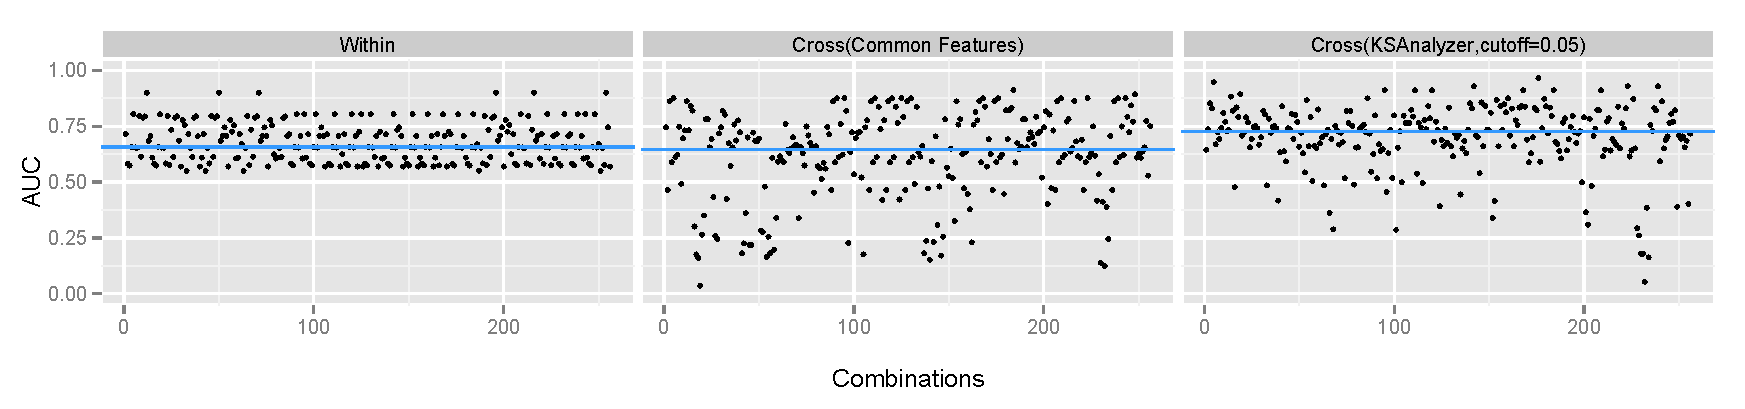
\includegraphics[width=\linewidth]{Figures/Result/auc_compare.pdf}
% 	\caption{Prediction performance variance among within-prediction,
% 	cross-prediction using common metrics, and cross-prediction by KSAnalyzer with
% 	the cutoff of 0.05 in terms of AUC. The number of prediction combinations is 256.}
% 	\label{fig:compare_results_on_defect}
% \end{figure*}


Table~\ref{tab:result_overview} shows the prediction performance (a median AUC)
of baselines and HDP by KSAnalyzer with the cutoff of 0.05 and Cliff's $\delta$ with its magnitude
for each target. The last row, {\em All} targets, show an overall prediction performance of baslines and HDP in a median AUC. Baseline1 represents
the WPDP results of a target project and Baseline2 shows
the CPDP results using common metrics (CPDP-CM) between source and target
projects. Baseline3 shows the results of CPDP-IFS proposed by He et
al.~\cite{He14} and Baseline4 represents the UDP results by CLAMI~\cite{nam2015clami}.
The last column shows the HDP results by KSAnalyzer with the cutoff of 0.05. If there are better results between Baseline1 and our approach with statistical significance (Wilcoxon signed-rank
test~\cite{Wilcoxon45}, p$<$0.05), the better AUC values are in
bold font as shown in Table~\ref{tab:result_overview}.
Between Baseline2 and our approach, better AUC values with
statistical significance are underlined in
the table. Between Baseline3 and our approach, better AUC values with
statistical significance are shown with an asterisk (*).
Between Baseline4 and our approach, better AUC values with
statistical significance are shown with an ampersand ($^{\&}$).

The values in parentheses in Table~\ref{tab:result_overview} show Cliff's $\delta$ and its magnitude for the effect size among baselines and HDP. If a Cliff's $\delta$ is a positive value, HDP improves a baseline in terms of the effect size. As explained in Section~\ref{sec:measure}, based on a Cliff's $\delta$, we can estimate the magnitude of the effect size (N: Negligible, S: Small, M: Medium, and L: Large). For example, the Cliff's $\delta$ of AUCs between WPDP and HDP for pc5 is 0.828 and its magnitude is {\em Large} as in Table~\ref{tab:result_overview}. In other words, HDP outperforms WPDP in pc5 with the large magnitude of the effect size.

%From Table~\ref{tab:result_overview},
We observed the following results about RQ1:
\squishlist
	\item The 18 out of 34 targets (Safe, ZXing, ant-1.3, arc, camel-1.0, poi-1.5, skarbonka, xerces-1.2, mw1, pc2, pc5, mc1, mc2, kc3, ar1, ar3, ar4, and ar5) show better with statistical significance or comparable results against WPDP.
  However, HDP by KSAnalyzer with the cutoff of
	0.05 did not lead to better with statistical
	significance or comparable against WPDP in {\em All} in our empirical settings. Note that WPDP is an upper bound of prediction performance. In this sense, HDP shows potential when there are no training datasets with the same metric sets as target datasets.
	\item The Cliff's $\delta$ values between WPDP and HDP are positive in 14 out of 34 targets. In about 41\% targets, HDP shows negligible or better results to HDP in terms of effect size.
	\item HDP by KSAnalyzer with the cutoff of 0.05
	leads to better or comparable results to CPDP-CM
	with statistical significance. (no underlines in CPDP-CM of
	Table~\ref{tab:result_overview})
	\item HDP by KSAnalyzer with the cutoff of 0.05 outperforms
	CPDP-CM with statistical significance
	when considering results from {\em All} targets in our experimental
	settings.
	\item The Cliff's $\delta$ values between CPDP-CM and HDP are positive in 30 out 34 targets. In other words, HDP improves CPDP-CM in most targets in terms of effect size.
	\item HDP by KSAnalyzer with the cutoff of 0.05
	leads to better or comparable results to CPDP-IFS with
	statistical significance. (no asterisks in CPDP-IFS of
	Table~\ref{tab:result_overview})
	\item HDP by KSAnalyzer with the cutoff of 0.05 outperforms
	CPDP-IFS with statistical significance
	when considering results from {\em All} targets in our experimental
	settings.
	\item The Cliff's $\delta$ values between CPDP-IFS and HDP are positive in all targets except for velocity-1.4.
  \item HDP by KSAnalyzer with the cutoff of 0.05 outperforms
	UDP with statistical significance
	when considering results from {\em All} targets in our experimental
	settings.
	\item The magnitude of Cliff's $\delta$ values between UDP and HDP are negligible or positively better in 29 out 34 targets.
\squishend

%%%%%%%%%%%%%%%%%%%%%%%%%%%%%%%%%%%%%%%%
%%%%%%%%%%%%%%%%%%%%%%%%%%%%%%%%%%%%%%%%
%%%%%%%%%%%%%%%%%%%%%%%%%%%%%%%%%%%%%%%%
%%%%%%%%%%%%%%%%%%%%%%%%%%%%%%%%%%%%%%%%

\subsection{Target Prediction Coverage}
\label{subsec02}
Target prediction coverage shows how many target projects can be
predicted by the HDP models. If there are no feasible prediction
combinations for a target because of there being no matched metrics
between source and target datasets, it might be difficult to use an HDP model in
practice.

\begin{table}[t]
%\small
%\scriptsize
\centering
\caption{Median AUCs of baselines and
HDP in KSAnalyzer (cutoff=0.05) by each source group.
% Cross-results by analyzer are compared to
% those of using common features as well. Outperforming results with statistical
% significance (Wilcoxon signed-rank test, p$<$0.05) between within and cross by
% the proposed approach and between cross using common features and those by the
% proposed approach are bold-faced and underlined respectively.
}
\label{tab:compare}
%\begin{tabular}{|@{ }c@{ }||@{ }c@{ }|@{ }c@{ }|@{ }c@{ }|@{ }c@{ }||@{ }c@{ }|}
\begin{tabular}{|@{ }c@{ }|@{ }c@{ }|@{ }c@{ }|@{ }c@{ }|@{ }c@{ }|@{ }c@{ }||@{ }c@{ }|}
\hline

% \multirow{2}{*}{\specialcell{{\bf Source}\\{\bf group}}}	&
% \multirow{2}{*}{{\bf Within}} &
% \multicolumn{3}{c|}{{\bf Cross}}	&
% \multirow{2}{*}{\specialcell{{\bf Target}\\{\bf coverage}}}
{\bf Source}
%& \specialcell{{WPDP}|\\{(Baseline1)}}
%& \specialcell{{CPDP-CM}\\{(Baseline2)}}
%& \specialcell{{CPDP-IFS}\\{(Baseline3)}}
%& \specialcell{{UDP}\\{(Baseline4)}}
& WPDP
& CPDP-CM
& CPDP-IFS
& UDP
& \specialcell{{HDP}\\{KS,0.05}}
& \specialcell{{Target}\\{Coverage}\\{of HDP}} \\ \hline \hline
%AEEEM & 0.654	& 0.736 &0.528	& {\bf 0.739}* & 48\%\\
AEEEM       &0.732  &0.750  &0.722  &0.776  &0.753    &35\%\\ \hline %10/29
%& 80\\  \hline
%ReLink & 0.654	& 0.665 &0.500	& 0.702* & 88\% \\ \hline		%& 37\\ \hline
Relink      &{\bf 0.731}    &0.655  &0.500  &0.683  &\underline{0.694}*      &84\%\\ \hline %26/31
%MORPH & 0.657	& 0.667 &0.590	& {\bf \underline{0.736}}* & 100\% \\ \hline	 %&
MORPH       &0.741  &0.652  &0.589  &0.732  &\underline{0.724}*     &92\%\\ \hline	%22/24
% 100\\
% \hline
%NASA & 0.654	& 0.527	&0.500	& \underline{{\bf 0.734}}* &  52\% \\ \hline		%&
NASA        &0.732  &0.550  &0.541  &0.754  &\underline{0.734}*       &100\%\\ \hline %23
% 70\\
% \hline
%SOFTLAB & 0.695	& 0.612	&0.554	& \underline{0.708}* & 100\% \\ \hline%\hline	%&
SOFTLAB     &{\bf 0.741}    &0.631  &0.551  &0.681  &\underline{0.692}*      &100\%\\ \hline	%29
% 29\\
% \hline\hline
%\bf{\emph{All}} &  0.657 & 0.636 & \underline{\bf 0.724} & 100\%\\	%& 316\\
%\hline

%{\bf Non-defect All} &{\bf 0.67}	&{\bf 0.73}	&{\bf 0.61} &  \\ \hline


\end{tabular}
\end{table}
For target prediction coverage, we analyzed our HDP results by KSAnalyzer with
the cutoff of 0.05 by each source group. For example, after applying
metric selection and matching, we can build a prediction model by using EQ in
AEEEM and predict each of 29 target projects in four other dataset
groups. However, because of the cutoff value, some predictions may not be
feasible. For example, EQ$\Rightarrow$Apache was not feasible because there are
no matched metrics whose matching scores are greater than 0.05.
Instead, another source dataset, JDT, in AEEEM has
matched metrics to Apache. In this case, we consider
the source group, AEEEM, covered Apache. In other words, if
any dataset in a source group can be used to build an HDP model for a target, we
count the target prediction is as covered.

Table~\ref{tab:compare} shows the median AUCs and
prediction target coverage. The median AUCs were computed by the AUC
values of the feasible HDP predictions and their corresponding predictions of
WPDP, CPDP-CM, CPDP-IFS, and UDP. We conducted the Wilcoxon
signed-rank test on results between WPDP and baselines~\cite{Wilcoxon45}. Like
Table~\ref{tab:result_overview}, better results between baselines and our
approach with statistical significance are in bold font, underlined, with asterisks and/or with
ampersands.% in Table~\ref{tab:compare} accordingly.

First of all, in each source group, we could observe WPDP did not outperform HDP in three source groups, AEEEM, MORPH, and NASA, with statistical significance.
For example, target projects were predicted by some projects in AEEEM and
the median AUC for HDP by KSAnalyzer is 0.753 while that of
WPDP is 0.732. In addition,
HDP by KSAnalyzer also
outperforms CPDP-CM and CPDP-IFS.
There are no better results in CPDP-CM
than those in HDP by KSAnalyzer with statistical significance (no
underlined results in third column in Table~\ref{tab:compare}). In addition, HDP
by KSAnalyzer outperforms CPDP-IFS in most source groups with statistical significance except for AEEEM. Between UDP and HDP, we did not observe significant performance difference as there are no ampersands in any AUC values in both UDP and HDP.

The target prediction coverage in the NASA and SOFTLAB groups yielded 100\% as
shown in Table~\ref{tab:compare}. This implies our HDP models may conduct defect
prediction with high target coverage even using datasets which only appear in
one source group. AEEEM, ReLink, and MORPH groups have 35\%, 84\%, and 92\% respectively
since some prediction combinations do not have matched metrics because of low matching scores ($\leq$0.05).
Thus, some prediction combinations
using matched metrics with low matching scores can be automatically excluded. In
this sense, our HDP approach follows a similar concept to the two-phase
prediction model~\cite{Kim13}: (1) checking prediction feasibility between
source and target datasets, and (2) predicting defects.

%%%%%%%%%%%%%%%%%%%%%%%%%%%%%%%%%%%%%%%%
%%%%%%%%%%%%%%%%%%%%%%%%%%%%%%%%%%%%%%%%
%%%%%%%%%%%%%%%%%%%%%%%%%%%%%%%%%%%%%%%%
%%%%%%%%%%%%%%%%%%%%%%%%%%%%%%%%%%%%%%%%

\subsection{Win/Tie/Loss Results}
\label{subsec03}
\begin{table*}[!t]
%\small
%\scriptsize
\centering
\caption{Win/Tie/Loss results of HDP by KSAnalyzer (cutoff=0.05)
against WPDP (Baseline1), CPDP-CM (Baseline2), and CPDP-IFS (Baseline3).}
\label{tab:win_results}
%\setlength{\tabcolsep}{5pt}
%\setlength{\extrarowheight}{1.5pt}
%\begin{tabular}{|@{ }c@{ }||@{ }c@{ }|@{ }c@{ }|@{ }c@{ }||@{ }c@{ }|@{ }c@{
%}|@{ }c@{ }|}
%\begin{tabular}{|@{}c@{}||@{}c@{}|@{}c@{}|@{}c@{}||@{}c@{}|@{}c@{}|@{}c@{}||@{}c@{}|@{}c@{}|@{}c@{}||@{}c@{}|@{}c@{}|@{}c@{}|}
\begin{tabular}{|c||c|c|c||c|c|c||c|c|c||c|c|c|}
\hline

\multirow{3}{*}{{\bf Target}}
&\multicolumn{12}{c|}{\bf Against}
\\ \cline{2-13}
&\multicolumn{3}{c||}{\specialcell{{\bf WPDP}\\{(Baseline1)}}}
&\multicolumn{3}{c||}{\specialcell{{\bf CPDP-CM}\\{(Baseline2)}}}
&\multicolumn{3}{c||}{\specialcell{{\bf CPDP-IFS}\\{(Baseline3)}}}
&\multicolumn{3}{c|}{\specialcell{{\bf UDP}\\{(Baseline4)}}}
\\
\cline{2-13}

& Win & Tie & Loss & Win & Tie & Loss & Win & Tie & Loss & Win & Tie & Loss \\ \hline \hline
EQ  &0      &0      &4      &1      &2      &1      &4      &0      &0      &3      &0      &1\\ \hline
    JDT &0      &0      &5      &3      &0      &2      &5      &0      &0      &4      &0      &1\\ \hline
    LC  &0      &0      &7      &3      &3      &1      &3      &1      &3      &0      &0      &7\\ \hline
    ML  &0      &0      &6      &4      &2      &0      &6      &0      &0      &6      &0      &0\\ \hline
    PDE &0      &0      &5      &2      &0      &3      &5      &0      &0      &4      &0      &1\\ \hline
    Apache      &4      &0      &8      &8      &0      &4      &10     &0      &2      &4      &0      &8\\ \hline
    Safe        &11     &1      &7      &14     &0      &5      &17     &0      &2      &15     &1      &3\\ \hline
    ZXing       &5      &0      &0      &4      &0      &1      &4      &0      &1      &4      &1      &0\\ \hline
    ant-1.3     &5      &1      &5      &7      &0      &4      &9      &0      &2      &6      &0      &5\\ \hline
    arc &0      &0      &3      &2      &0      &1      &3      &0      &0      &3      &0      &0\\ \hline
    camel-1.0   &2      &0      &5      &5      &0      &2      &6      &0      &1      &3      &0      &4\\ \hline
    poi-1.5     &2      &0      &2      &3      &1      &0      &2      &0      &2      &2      &0      &2\\ \hline
    redaktor    &0      &0      &4      &2      &0      &2      &3      &0      &1      &3      &0      &1\\ \hline
    skarbonka   &15     &0      &0      &5      &1      &9      &13     &0      &2      &2      &0      &13\\ \hline
    tomcat      &0      &0      &1      &1      &0      &0      &1      &0      &0      &1      &0      &0\\ \hline
    velocity-1.4        &0      &0      &6      &2      &0      &4      &2      &0      &4      &2      &0      &4\\ \hline
    xalan-2.4   &0      &0      &1      &0      &0      &1      &1      &0      &0      &0      &0      &1\\ \hline
    xerces-1.2  &1      &0      &1      &2      &0      &0      &1      &0      &1      &2      &0      &0\\ \hline
    cm1 &0      &1      &9      &8      &0      &2      &9      &0      &1      &7      &0      &3\\ \hline
    mw1 &4      &0      &3      &5      &0      &2      &5      &0      &2      &5      &0      &2\\ \hline
    pc1 &0      &0      &7      &6      &0      &1      &7      &0      &0      &7      &0      &0\\ \hline
    pc3 &0      &0      &7      &7      &0      &0      &7      &0      &0      &7      &0      &0\\ \hline
    pc4 &0      &0      &8      &5      &0      &3      &8      &0      &0      &6      &0      &2\\ \hline
    jm1 &1      &0      &5      &5      &0      &1      &6      &0      &0      &5      &0      &1\\ \hline
    pc2 &4      &0      &1      &5      &0      &0      &5      &0      &0      &5      &0      &0\\ \hline
    pc5 &1      &0      &0      &1      &0      &0      &1      &0      &0      &1      &0      &0\\ \hline
    mc1 &1      &0      &0      &1      &0      &0      &1      &0      &0      &1      &0      &0\\ \hline
    mc2 &10     &2      &6      &15     &0      &3      &14     &0      &4      &8      &2      &8\\ \hline
    kc3 &9      &0      &2      &8      &0      &3      &10     &0      &1      &9      &0      &2\\ \hline
    ar1 &12     &0      &2      &12     &1      &1      &10     &0      &4      &12     &0      &2\\ \hline
    ar3 &15     &0      &2      &8      &0      &9      &11     &2      &4      &15     &0      &2\\ \hline
    ar4 &6      &1      &10     &15     &1      &1      &16     &0      &1      &13     &2      &2\\ \hline
    ar5 &15     &0      &7      &15     &0      &7      &15     &0      &7      &14     &1      &7\\ \hline
    ar6 &5      &0      &11     &10     &3      &3      &13     &0      &3      &5      &3      &8\\ \hline
    Total       &\specialcell{{128}\\{45.1\%}}  &\specialcell{{6}\\{2.1\%}}     &\specialcell{{150}\\{52.8\%}}  &\specialcell{{194}\\{68.3\%}}  &\specialcell{{14}\\{4.9\%}}    &\specialcell{{76}\\{26.8\%}}   &\specialcell{{233}\\{82.0\%}}  &\specialcell{{3}\\{1.1\%}}     &\specialcell{{48}\\{16.9\%}}   &\specialcell{{184}\\{64.8\%}}  &\specialcell{{10}\\{3.5\%}}    &\specialcell{{90}\\{31.7\%}}\\ \hline
%Total & \specialcell{{147}\\{66.2\%}} &\specialcell{{3}\\{1.4\%}}
%&\specialcell{{72}\\{32.4\%}}
%& \specialcell{{147}\\{66.2\%}} &\specialcell{{14}\\{6.3\%}}
%&\specialcell{{61}\\{27.5\%}}
%& \specialcell{{182}\\{82.0\%}} &\specialcell{{3}\\{1.3\%}}
%&\specialcell{{37}\\{16.7\%}}
%\\
%\hline
\end{tabular}
\end{table*}


To investigate the evaluation results for HDP in detail, we report
the Win/Tie/Loss results of HDP by KSAnalyzer with the cutoff of 0.05 against
WPDP (Baseline1), CPDP-CM (Baseline2), CPDP-IFS (Baseline3), and UDP (Baseline4) in Table~\ref{tab:win_results}.


KSAnalyzer with the cutoff of 0.05 conducted 284 out of 962 prediction
combinations since 678 combinations do not have any matched
metrics because of the cutoff threshold. In
Table~\ref{tab:win_results}, the target dataset, ZXing, was predicted in five
prediction combinations and our approach, HDP, outperforms Baselines in the four or five combinations (i.e. 4 or 5 Wins). However, CPDP-CM and CPDP-IFS outperform HDP in one combination of the target, ZXing (1 Loss).


% \subsection{Matched features}
% In this section, we discuss matched features to investigate prediction
% performance on cross-domain defect prediction in detail.

% A reason why ASAnalyzer can predict defects pretty well on cross-domain
% settings is that most defect prediction metrics usually represent complexity of
% source code and its change; it tends to be more buggy when the complexity is
% higher.
Against Baseline1, the four targets such as ZXing, skarbonka, pc5, and mc1 have only Win results. In other words, defects in those four targets
could be predicted better by other source projects using HDP models by
KSAnalyzer compared to WPDP models.

\label{sec:why}
\begin{figure}[t]
	\centering
	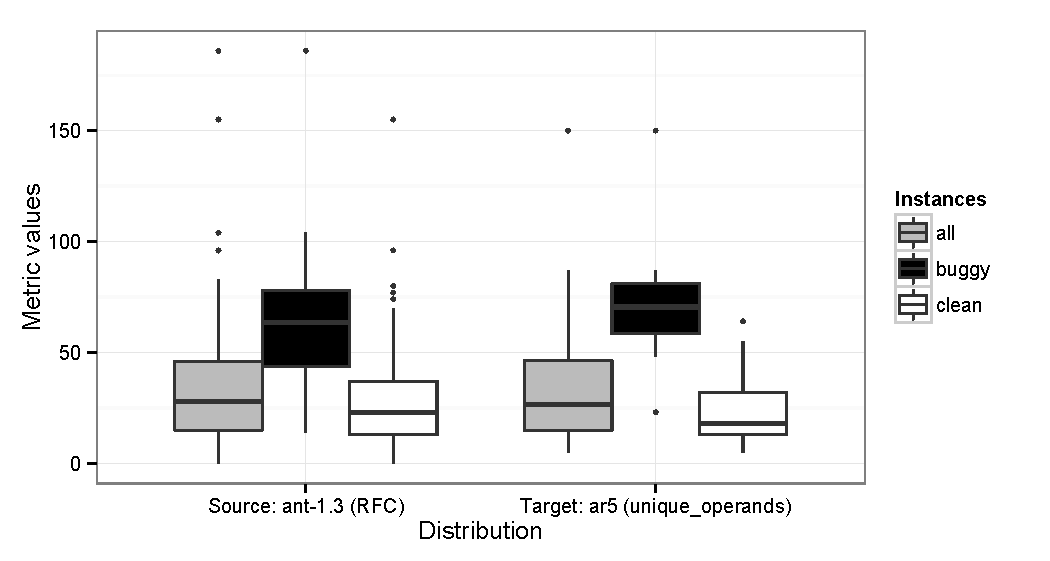
\includegraphics[width=\linewidth]{Figures/Result/best_dist_bplot.pdf}
	\caption{Distribution of metrics (matching score=0.91)
	from ant-1.3$\Rightarrow$ar5 (AUC=0.946).}
	\label{fig:best_dist}
\end{figure}

In Figure~\ref{fig:best_dist}, we analyzed distributions of matched metrics using box plots for one of Win cases, ant-1.3$\Rightarrow$ar5.
% the feature value distribution of
% a matched feature in the prediction combination, ant-1.3$\Rightarrow$ar5, whose AUC is 0.938.
The gray, black, and white box plots show distributions of matched metric values in
all, buggy, and clean instances respectively. The three box plots on the
left-hand side represent distributions of a source metric while the three
box plots on the right-hand side represent those of a target metric. The
bottom and top of the boxes represent the first and third quartiles
respectively.
The solid horizontal line in a box represents the median metric value in each distribution.
Black points in the figure are outliers.

Figure~\ref{fig:best_dist} explains how the prediction
combination of ant-1.3$\Rightarrow$ar5 can have a high AUC, 0.946. Suppose
that a simple model predicts that an instance is buggy when the metric value of
the instance is more than 40 in the case of Figure~\ref{fig:best_dist}. In both
datasets, approximately 75\% or more buggy and clean instances will be
predicted correctly. In Figure~\ref{fig:best_dist}, the matched metrics in
ant-1.3$\Rightarrow$ar5 are the response for class ({\em RFC}: number of methods
invoked by a class)~\cite{Chidamber94} and the number of unique operands ({\em
unique\_operands})~\cite{Halstead77}, respectively. The {\em RFC} and {\em
unique\_operands} are not the same metric so it might look like an arbitrary
matching. However, they are matched based on their similar distributions as
shown in Figure~\ref{fig:best_dist}. Typical defect prediction metrics have
tendencies in which higher complexity causes more
defect-proneness~\cite{DAmbros12,Menzies07,Rahman13}. In
Figure~\ref{fig:best_dist}, instances with higher values of {\em RFC} and {\em
unique\_operands} have the tendency to be more defect-prone. For this reason, the
model using the matched metrics could achieve such a high AUC (0.946). We could
observe this defect-proneness tendency in other Win results (See the online appendix, https://lifove.github.io/hdp/\#pc). Since matching metrics is
based on similarity of source and target metric distributions, HDP also
addresses several issues related to a dataset shift such as the covariate shift
and domain shift discussed by Turhan~\cite{Turhan12}.

%The Win/Tie/Loss results show that with our HDP model by KSAnalyzer there is a higher possibility of getting a better prediction performance.


%%%%%%%%
% LOSS results
%%%%%%%
However, there are still about 52.8\% Loss results against WPDP as shown in Table~\ref{tab:win_results}. The 14 targets have no Wins at all against Baseline1. In
addition, other targets still have Losses even though they have Win or Tie
results.


\begin{figure}[t]
	\centering
	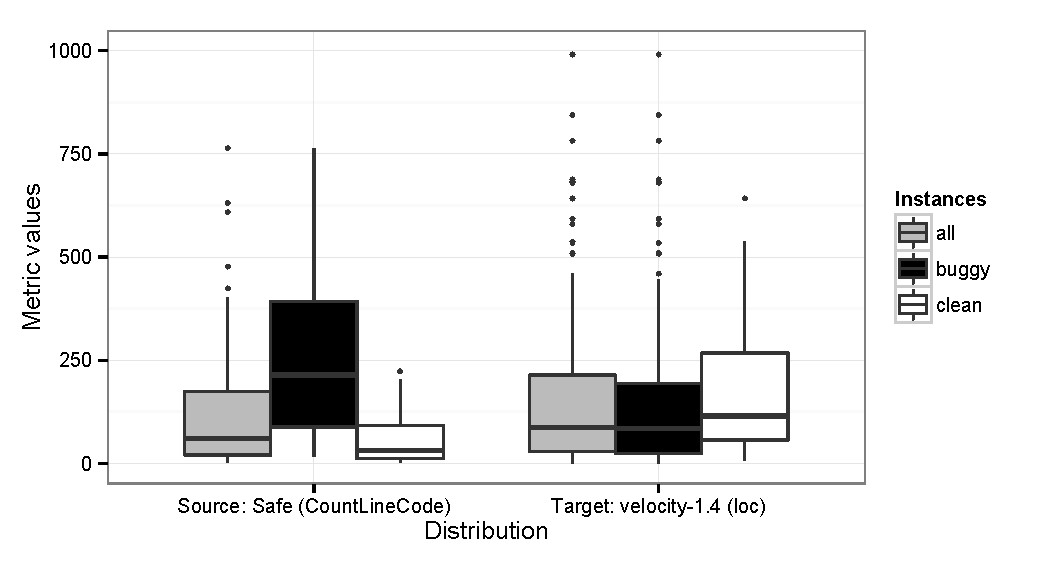
\includegraphics[width=\linewidth]{Figures/Result/loss_dist_bplot.pdf}
	\caption{Distribution of metrics (matching score=0.45)
	from Safe$\Rightarrow$velocity-1.4 (AUC=0.391).}
	\label{fig:loss_dist}
\end{figure}


As a representative Loss case, we investigated distributions of the matched metrics in Safe$\Rightarrow$velocity-1.4, whose AUC is 0.391.
As observed, Loss results were usually caused by different tendencies of
defect-proneness between source and target metrics. Figure~\ref{fig:loss_dist}
shows how the defect-prone tendencies of source and target metrics are different.
Interestingly, the matched source and target metric by the KSAnalyzer is the
same as {\em LOC} ({\em CountLineCode} and {\em loc}) in both.
As we observe in the figure, the median metric value of buggy instances is higher than that of clean instances in that the more {\em LOC}
implies the higher defect-proneness in the case of Safe. However, the median metric value of
buggy instances in the target is lower than that of clean instances
in that the less {\em LOC} implies the higher defect-proneness in
velocity-1.4. This inconsistent tendency of
defect-proneness between the source and target metrics could degrade the
prediction performance although they are the same metric.

We regard the matching that has an inconsistent defect-proneness tendency between
source and target metrics as {\em a noisy metric matching}.
% This implies the target
% feature does not follow the tendency that a higher complexity causes more defect-proneness.
% The target feature worked as noise when the model predicted
% defects in velocity-1.4.
We could observe this kind of noisy metric matching in
prediction combinations in other Loss results.

However, it is very challenging to filter out the noisy metric matching since we
cannot know labels of target instances in
advance. If we could design a filter for the noisy metric matching, the Loss
results would be minimized. Thus, designing a new filter to mitigate these Loss
results is an interesting problem to address. Investigating this new filter
for the noisy metric matching will remain as future work.

Figure~\ref{fig:loss_dist} also explains why CPDP-CM did not show reasonable
prediction performance. Although the matched metrics are same
as {\em LOC}, its defect-prone tendency is inconsistent. Thus, this matching using
the common metric was noisy and was not helpful for building a prediction model.

% The DM filter could not remove
% this matched feature since the modality of all instances in both source and
% target is still similar. Without knowing labels of target instances, it is
% difficult to filter out this case. Other Loss results also have similar
% observations. Designing new filters for these Loss results is a challenging
% issue since we cannot know distribution of clean and buggy instances of target in
% advance. Investigating new filters for these patterns remains as future work.



% The pc4 in Table~\ref{tab:win_results} also have many Loss results.
% However, note that pc4 still have very high AUC values, 0.899 and 0.70,
% respectively, The AUC value of 0.70 is considered as a promising result in defect prediction~\cite{Giger12, Lessmann08}. The reason for Loss results
% of pc1 and pc3 is that within-results in AUC are already very high, 0.78 and
% 0.79, respectively.


%\TODO{Guidelines or suggestions on cross-domain defect prediction?}

Overall, the numbers of Win and
Tie results are 128 and 6 respectively out of all 284 prediction
combinations.
This means that in 47.1\% of prediction combinations our HDP
models achieve better or comparable prediction performance than those in
WPDP.

However, HDP show relatively better results against Baseline2, Baseline3, and Baseline4 in terms of the Win/Tie/Loss evaluation.
In the 208 (73.2\%) out of 284 prediction combinations, HDP outperforms and is comparable to CPDP-CM. Against Baseline3, 236
(83.1\%) prediction combinations are Win or Tie results. Against Baseline4, HDP has 194 Win or Tie results (68.3\%).

%A recent study shows that high defect rate of a dataset may bias prediction results,i.e., higher buggy rate of a dataset tends to lead better prediciton results~\cite{Tantithamthavorn16}. This bias could be matter under the WPDP setting as the study discusses about model validation technioques~\cite{Tantithamthavorn16}. Since HDP is CPDP on datasets using different metric sets, To make sure if the promising reuslts of HDP is affected by the defect rate of a target dataset


\subsection{Performance by Source Datasets}
\label{subsec04-0}

\begin{table}[!t]
\caption{HDP Prediction performance in median AUC by source datasets.}
\label{tab:by_source}
\begin{tabular}{|c||c|c||c||c|c|}
\hline
\bf{Source}	& \bf{AUC} 	&\specialcell{\bf{\# of}\\\bf{Targets}} &\bf{ Source} & \bf{AUC} 	&\specialcell{\bf{\# of}\\\bf{Targets}} \\ \hline
\hline
EQ	&0.794	&5	&JDT	&0.756	&10	\\ \hline
LC	&0.674	&2	&ML	&0.714	&3	\\ \hline
PDE	&n/a	&0	&Apache	&0.720	&17	\\ \hline
Safe	&0.684	&22	&ZXing	&0.707	&12	\\ \hline
ant-1.3	&0.738	&16	&arc	&0.666	&8	\\ \hline
camel-1.0	&0.803	&2	&poi-1.5	&0.761	&6	\\ \hline
redaktor	&n/a	&0	&skarbonka	&0.692	&17	\\ \hline
tomcat	&0.739	&9	&velocity-1.4	&n/a	&0	\\ \hline
xalan-2.4	&0.762	&7	&xerces-1.2	&n/a	&0	\\ \hline
cm1	&0.630	&9	&mw1	&0.710	&13	\\ \hline
pc1	&0.734	&9	&pc3	&0.786	&9	\\ \hline
pc4	&n/a	&0	&jm1	&0.678	&8	\\ \hline
pc2	&0.822	&3	&pc5	&n/a	&0	\\ \hline
mc1	&0.856	&3	&mc2	&0.739	&20	\\ \hline
kc3	&0.689	&5	&ar1	&0.320	&3	\\ \hline
ar3	&0.740	&11	&ar4	&0.674	&18	\\ \hline
ar5	&0.691	&28	&ar6	&0.740	&9	\\ \hline
\end{tabular}
\end{table}

Table~\ref{tab:by_source} shows prediction performance of HDP (KSAnalyzer, cutoff=0.05, and Gain Ratio feature selection) by each source dataset. The 3rd and 6th columns represent the number of targets predicted by a source. For example, EQ predicts five targets by HDP and the median AUC from these five target predictions is 0.794. Since the total number of feasible target predictions is 284 out of all 962 prediction combinations, six source datasets (PDE, redaktor, velocity-1.4, xerces-1.2, pc4, and pc5) did not predict any targets because there were no matched metrics.

The higher defect ratio of a training dataset may make bias as the prediction performance of the dataset with the higher defect ratio may be better than that with the lower defect ratio~\cite{Tantithamthavorn16}. To investigate if HDP is also affected by defect ratio of the training dataset and what makes better prediction performance, we analyzed the best and worst source datasets that lead to the best and worst AUC values, respectively.

We found that HDP does not bias prediction performance from the defect ratios of datasets and prediction performance is highly depending on the defect-proneness tendency of matched metrics under our experiments.
As shown in Table~\ref{tab:by_source}, the best source dataset is mc1 (0.856) although its defect ratio is very low, 0.73\%. We investigate distributions of matched metrics of EQ like Figure~\ref{fig:best_dist} and~\ref{fig:loss_dist}.\footnote{For detailed target prediction results and distributions of matched metrics by each source dataset, please refer to the online appendix: https://lifove.github.io/hdp/\#pc.} We observed that all the matched metrics for the source, EQ, show the typical defect-proneness tendency similarly to Figure~\ref{fig:best_dist}. The worst source dataset is ar1 (0.320) whose defect ratio is 7.44\%. We observed that the matched metrics of ar1 show inconsistent tendency of defect-proneness between source and target, i.e., noisy metric matching. From these best and worst cases, we confirm again the consistent defect-proneness tendency of matched metrics between source and target datasets is most important to lead to better prediction performance.






\begin{table*}[h]
%\small
%\scriptsize
\centering
\caption{Prediction performance (a
median AUC and \% of Win) in different metric selections.
% Between within- and
% cross-results by
% analyzers, outperforming results with statistical significance
% (Wilcoxon signed-rank, p$<$0.05) is bold-faced. Between cross-results using
% common features and by analyzers, outperforming results with
% statistical significance (Wilcoxon signed-rank, p$<$0.05) is underlined.}
}
\label{tab:various_fs}
%\setlength{\tabcolsep}{5pt}
%\setlength{\extrarowheight}{1.5pt}
%\begin{tabular}{|@{}c@{}||c@{ }|c@{}||c@{ }|c@{}||c@{ }|c@{}||c@{ }|c@{}||c|}
\begin{tabular}{|c||c|c||c|c||c|c||c|c||c|}
\hline
\multirow{3}{*}{\bf{Approach}}
&\multicolumn{8}{@{ }c@{ }||}{\bf Against}
&\multirow{2}{*}{\specialcell{\bf{HDP}}}
\\\cline{2-9}
&\multicolumn{2}{@{ }c@{ }||}{\specialcell{\bf{WPDP}}}
&\multicolumn{2}{@{ }c@{}||}{\specialcell{\bf{CPDP-CM}}}
&\multicolumn{2}{@{ }c@{ }||}{\specialcell{\bf{CPDP-IFS}}}
&\multicolumn{2}{@{ }c@{ }||}{\specialcell{\bf{UDP}}}
&
\\
\cline{2-10}
& \bf{AUC}
& \bf{Win\%}
& \bf{AUC}
& \bf{Win\%}
& \bf{AUC}
& \bf{Win\%}
& \bf{AUC}
& \bf{Win\%}
& \bf{AUC}
\\
\hline
\hline
Gain Ratio	& {\bf 0.732} &45.1\%	&0.632 &68.3\% &0.558 &82.0\% &0.702 &64.8\% &\underline{0.711}*$^{\&}$	\\ \hline
Chi-Square	& {\bf 0.741} &43.0\%	&0.635 &77.5\% &0.557 &83.3\% &0.720$^{\&}$ &65.2\% &\underline{0.717}*  \\ \hline
Significance& {\bf 0.734} &43.8\%	&0.630 &69.7\% &0.557 &83.4\% &0.693 &67.6\% &\underline{0.713}*$^{\&}$  \\ \hline
Relief-F		& {\bf 0.740} &42.4\%	&0.642 &66.2\% &0.540 &80.8\% &0.720  &62.6\%  &\underline{0.706}*	\\ \hline
None			& 0.657 &46.7\%	&0.622 &51.6\% &0.545 &64.2\% &0.693$^{\&}$ &44.0\% &\underline{{\bf 0.665}}*	\\ \hline
\end{tabular}
\end{table*}

\begin{table*}[ht]
%\footnotesize
%\scriptsize
\centering
\caption{Prediction performance in other analyzers with the matching
score cutoffs, 0.05 and 0.90.
% Between within- and
% cross-results by
% analyzers, outperforming results with statistical significance
% (Wilcoxon signed-rank, p$<$0.05) is bold-faced. Between cross-results using
% common features and by analyzers, outperforming results with
% statistical significance (Wilcoxon signed-rank, p$<$0.05) is underlined.}
}
\label{tab:other_analyzers}
%\setlength{\tabcolsep}{5pt}
%\setlength{\extrarowheight}{1.5pt}
%\begin{tabular}{|@{ }c@{ }|@{ }c@{ }||@{ }c@{ }||@{ }c@{ }|@{ }c@{ }|@{ }c@{
%}||@{ }c@{ }||@{ }c@{ }|@{ }c@{ }|@{ }c@{ }||@{ }c@{ }||@{ }c@{ }|}
%\begin{tabular}{|@{}c@{}|@{}c@{}||@{}c@{}|@{}c@{}||@{}c@{}|@{}c@{}||@{}c@{}|@{}c@{}||@{}c@{}||@{}c@{}|}
\begin{tabular}{|c|c||c|c||c|c||c|c||c|c||c|c|@{ }c@{ }|}
%\begin{tabular}{|c|c||F|F||F|F||F|F||F||c|}
\hline
\multirow{3}{*}{\specialcell{\bf{Analyzer}}}
&\multirow{3}{*}{\bf Cutoff}
&\multicolumn{8}{c||}{\bf Against}
&\multirow{2}{*}{\bf HDP}
&\multirow{3}{*}{\specialcell{\bf{Target}\\{\bf Coverage}}}
&\multirow{3}{*}{\specialcell{\bf{\# of Prediction}\\{\bf Combination}}}
\\ \cline{3-10}

&
&\multicolumn{2}{c||}{\specialcell{\bf{WPDP}}}
&\multicolumn{2}{c@{ }||}{\bf CPDP-CM}
&\multicolumn{2}{c@{ }||}{\bf CPDP-IFS}
&\multicolumn{2}{c@{ }||}{\bf UDP}
&
&
&
\\\cline{3-11}
&
& \bf{AUC}
& \bf{Win\%}
& \bf{AUC}
& \bf{Win\%}
& \bf{AUC}
& \bf{Win\%}
& \bf{AUC}
& \bf{Win\%}
& \bf{AUC}
&
&
\\
\hline
\hline
%PAnalyzer& 0.00 & \bf{0.684}	& \underline{0.640}	& 0.606 & 100\% \\ \hline
P& 0.05
& \bf{0.741} & 43.0\%
&0.655 & 54.9\%
&0.520	&69.5\%
&0.693$^{\&}$	&69.5\%
&0.642* & 100\%
&962
\\
\hline
P& 0.90
&{\bf 0.732} & 32.9\%
&0.629 & 62.9\%
&0.558	& 80.0\%
&0.680	& 59.3\%
& \underline{0.693}* & 100\%
&140
\\
\hline
\hline
\hline

%KSAnalyzer & 0.00 & 0.670 &	0.637	& \underline{0.669} & 100\% \\ \hline
KS & 0.05
&{\bf 0.732} & 45.1\%
&0.632 & 68.3\%
& 0.558	&82.0\%
& 0.702	&64.8\%
&\underline{0.711}*$^{\&}$ &100\%
& 284
\\\hline

KS& 0.90
& 0.816 & 55.6\%
&0.588 & 77.8\%
& 0.585	&100.0\%
& 0.786	&88.9\%
&\underline{0.831}* &21\%
& 90
\\ \hline
\hline
\hline

%SCoAnalyzer & 0.00 & \bf{0.684}	&\underline{0.640}	&0.517 & 100\% \\ \hline
SCo & 0.05
& \bf{0.741} & 16.9\%
&\underline{0.655} &41.9\%
& 0.520	&55.7\%
& 0.693$^{\&}$	&38.7\%
&0.609* & 100\%
& 962
\\
\hline
SCo& 0.90
& {\bf 0.741} & 17.7\%
&\underline{0.654} & 42.4\%
&0.520	&56.4\%
& 0.693$^{\&}$ &39.2\%
&0.614* &100\%
& 958
\\
\hline

%PiAnalyzer& 0.00 & \bf{0.684}	&\underline{0.640}	&0.589 & 100\% \\ \hline
% PiAnalyzer& 0.05 & \bf{0.684}	&0.582 &25.2\% & 100\% \\ \hline
% PiAnalyzer& 0.90 & \bf{0.684}	&0.592 &27.0\% & 100\% \\ \hline
\end{tabular}
\end{table*}

\subsection{Performance in Different Metric Selections}
\label{subsec04}

Table~\ref{tab:various_fs} shows prediction results on various metric selection approaches
including with no metric selection (`None'). We compare the median AUCs of
the HDP results by KSAnalyzer with the cutoff of 0.05 to those of WPDP, CPDP-CM,
CPDP-IFS, or UDP and report the percentages of Win results.

Overall, we could observe metric selection to be helpful in improving
prediction models in terms of AUC. When applying metric selection, the Win results
account for more than about 63\% in most cases against CPDP-CM and UDP. Against
CPDP-IFS, the Win results of HDP account for more than 80\% after applying the
metric selection approaches. This implies that the metric selection approaches
can remove irrelevant metrics to build a better prediction model.
%In addition, this result confirms
%the previous studies that we can build prediction models better than or
%comparable to WPDP models with even a few key metrics~\cite{Gao11, He14subset}.
However, the percentages of Win results in `None' were lower than those in
applying metric selection. Among metric selection approaches, `Gain Ratio', `Chi-Square' and
`Significance' based approaches lead to the best performance in terms of the
percentages of the Win results (64.8\%-83.4\%) against CPDP-CM, CPDP-IFS, and UDP.

\subsection{Performance in Various Metric Matching Analyzers}
\label{subsec05}

In Table~\ref{tab:other_analyzers}, we compare the prediction performance in
other analyzers with the matching score cutoff thresholds, 0.05 and 0.90.
HDP's prediction results by PAnalyzer, with a cutoff of 0.90, are
comparable to CPDP-CM and CPDP-IFS. This
implies that comparing 9 percentiles between source and target metrics can
evaluate the similarity of them well with a threshold of 0.90 against CPDP-CM and CPDP-IFS. However,
PAnalyzer with the cutoff is
too simple to lead to better prediction performance than KSAnalyzer. In
KSAnalyzer with a cutoff of 0.05, the AUC (0.711) better than that (0.693) of PAnalyzer with the cutoff of 0.90.

HDP by KSAnalyzer with a cutoff of 0.90 could show better AUC value (0.831) compared to that (0.711) with the
cutoff of 0.05.
However, the target coverage is just 21\%. This is because some prediction
combinations are automatically filtered out since poorly matched metrics, whose
matching score is not greater than the cutoff, are ignored. In other words,
defect prediction for 79\% of targets was not
conducted since the matching scores of matched metrics in prediction
combinations for the targets are not greater than 0.90 so
that all matched metrics in the combinations were ignored.

An interesting observation in PAnalyzer and KSAnalyzer is that AUC
values of HDP by those analyzers tend to be improved when a cutoff threshold
increased. As the cutoff threshold increased as 0.05, 0.10, 0.20,\ldots, and
0.90, we observed prediction results by PAnalyzer and KSAnalyzer
gradually are improved from 0.642 to 0.693 and 0.711 to 0.831 in AUC, respectively.
This means these two analyzers can filter out negative prediction combinations
well. As a result, the percentages of Win results are also increased.

HDP results by SCoAnalyzer were
worse than WPDP, CPDP-CM, and UDP. In addition,
prediction performance rarely changed regardless of cutoff thresholds; results
by SCoAnalyzer in different cutoffs from 0.05 to 0.90 did not
vary as well.
A possible reason is that SCoAnalyzer does not directly compare
the distributions between source and target metrics.
This result implies that the similarity of distribution between source and
target metrics is a very important factor for building a better
prediction model.


\subsection{Performance in Various Machine Learners}
\label{subsec06}
\begin{table*}[!t]
%\small
%\scriptsize
\centering
\caption{Prediction performance (a median AUC and \%
of Win) of HDP by KSAnalyzer (cutoff=0.05)
against WPDP, CPDP-CM, and CPDP-IFS by different machine learners.}
\label{tab:diff_learners}
%\setlength{\tabcolsep}{5pt}
%\setlength{\extrarowheight}{1.5pt}
%\begin{tabular}{|c||m{1.5cm}|m{1.5cm}|m{1.5cm}||m{1.5cm}|m{1.5cm}|m{1.5cm}|}
%\begin{tabular}{|@{ }c@{ }||c@{ }|@{ }c@{}||c@{ }|@{ }c@{ }||c@{ }|@{ }c@{}||c@{ }|}
\begin{tabular}{|c||c|c||c|c||c|c||c|c||c|}
\hline
\multirow{3}{*}{\specialcell{{\bf HDP}\\{\bf Learners}}}
&\multicolumn{8}{@{ }c@{ }||}{\bf Against}

&\multirow{2}{*}{{\bf HDP}}
\\ \cline{2-9}

&\multicolumn{2}{@{ }c@{ }||}{\specialcell{{\bf WPDP}}}
&\multicolumn{2}{@{ }c@{ }||}{\specialcell{{\bf CPDP-CM}}}
&\multicolumn{2}{@{ }c@{ }||}{\specialcell{{\bf CPDP-IFS}}}
&\multicolumn{2}{@{ }c@{ }||}{\specialcell{{\bf UDP}}}
&
\\
\cline{2-10}

&AUC & Win
&AUC & Win
&AUC & Win
&AUC & Win
&AUC
 \\ \hline \hline

SimpleLogistic	&0.763 &44.0\% 	&0.680 &60.9\%
&0.691 & 62.7\%  &0.734 & 48.9\%    	&\underline{0.718}*\\ \hline

RandomForest			&{\bf 0.732} &39.4\%		&0.629 &46.5\%
&0.619 & 63.0\% &0.674$^{\&}$ & 84.9\% 		&0.640*\\ \hline

BayesNet		&{\bf 0.703} &41.5\%		&0.583 &48.2\%
&0.675* & 29.2\% &0.666$^{\&}$ & 35.2\% 		&\underline{0.633} 	\\ \hline

%NaiveBayes		&26.1\%	&1.8\%	&71.1\% &54.5\% &3.2\% &42.3\%	\\ \hline

SVM				&0.500 &29.9\%		&0.500 &28.2\%
&0.500 &26.4\% &0.635$^{\&}$  &11.6\% 	&0.500 \\ \hline

J48				&{\bf 0.598} &34.2\%	&0.500 &44.7\%
&0.558 & 46.8\% &0.671$^{\&}$  & 18.7\% 			&\underline{0.568}   \\ \hline

Logistic			& {\bf 0.732} &45.1\%	&0.632 &68.3\%
&0.558 &82.0\% &0.702 &64.8\% &\underline{0.711}*$^{\&}$	\\ \hline

LMT				&{\bf 0.751} &42.3\% 	&0.671 &58.5\%
&0.690 &56.0\% &0.734$^{\&}$ &41.9\% 		&\underline{0.702}   \\ \hline

\end{tabular}
\end{table*}

To investigate if
HDP works with other machine learners, we built HDP models (KSAnalyzer and
the cutoff of 0.05) with various learners used in defect prediction
literature such as SompleLogistic, Random Forest, BayesNet, SVM, J48 Decision
Tree, and Logistic Model Trees
(LMT)~\cite{DAmbros12,Ghotra15,Lee11,Lessmann08,Nam13,Song11,Ghotra15}.
Table~\ref{tab:diff_learners} shows median AUCs and Win results.

Machine learners based on logit function such as SimpleLogistic, Logistic, and LMT led to the promising results among various learners (median AUC $>$ 0.70).
Logistic Regression uses the logit function and Simple Logistic builds a linear logistic regression model based on LogitBoost~\cite{Landwehr2005}.
LMT adopts Logistic Regression at the leaves of decision tree~\cite{Ghotra15}.
Thus, these learners work well when there is a linear
relationship between a predictor variable (a metric) and the logit
transformation of the outcome variable (defect-proneness)~\cite{Landwehr2005,Logstic}.
In our study, this linear relationship is related to the defect-proneness tendency of
a metric, that is, a higher complexity causes more defect-proneness~\cite{DAmbros12,Menzies07,Rahman13}.
As the consistent defect-prone tendency of matched metrics is important in HDP, the
HDP models built by  the logistic-based learners can lead to the promising prediction
performance.

%HDP models built by other learners such as
%Logistic and LMT led to comparable results to Simple Logistic against
%CPDP-CM and CPDP-IFS. Against Baseline2, Win + Tie results in
%Logistic and LMT are greater than about 70\%.
%Against Baseline3, the HPD results with Simple
%Logistic and LMT are similar to those with Logistic regression. In our experimental settings, HDP tends to
%work well with the learners based on the linear relationship between a metric
%and a label (defect-proneness).

According to the recent study by Ghotra et al., LMT and Simple Logistic tend to lead to better prediction performance than other kinds of machine learners~\cite{Ghotra15}. HDP results based on Simple Logistic and LMT also confirm the results by Ghotra et al.~\cite{Ghotra15}. However, these results do not generalize HDP works best by logistic-based learners as Ghotra et al. also pointed out prediction results and the best machine learner may vary based on each dataset~\cite{Ghotra15}.

There are several interesting observations in Table~\ref{tab:diff_learners}. SVM did not work for HDP and all baselines as their AUC values are 0.500.
This result also confirms the study by Ghotra et al. as SVM was ranked in the lowest group~\cite{Ghotra15}. Except for SimpleLogistic and Logistic, UDP outperforms HDP in most learners with statistical significance. CLAMI for UDP is also based on defect-proneness tendency of a metric~\cite{nam2015clami}. If target datasets follow this tendency very well, CLAMI could lead to promising prediction performance as CLAMI is not affected by the distribution differences between source and target datasets~\cite{nam2015clami}. Detailed comparison of UDP and HDP is an interesting future direction as UDP techniques have received much attention recently~\cite{nam2015clami,Zhang2016ICSE,Yang2016FSE}. We remain this detailed comparative study as future work.

\subsection{Summary}
In Section~\ref{sec:Result}, we showed HDP results for RQ1. The followings are the key observations of the results in our experimental setting:
\squishlist
    \item Overall, HDP led to better or comparable results to the baselines such as CPDP-CM, CPDP-IFS, and UDP when using the Logistic learner with KSAnalyzer (the cutoff of 0.05) and Gain ratio attribute selection.
    \item Compared to WPDP (0.732), HDP achieved 0.711 in terms of median AUC. Note that WPDP is an upper bound and 18 of 34 projects show better prediction results with statistical significance in terms of median AUC. However, there are still 52.8\% of Loss results against WPDP. Based on the analysis of distributions of matched metrics, we observed that the Loss cases are caused by the inconsistent defect-proneness tendency of the matched metrics. Identifying the inconsistent tendency in advance is a challenging problem to be solved.
    \item Applying metric selection approaches could improve HDP performances against the baselines.
    \item KSAnalyzer showed the best HDP performance compared to PAnalyzer and SCoAnalyzer. This confirms that KS-test is a good tool to decide whether distributions of two variables are drawn from the same distribution~\cite{Lilliefors67,Massey51}.
    \item HDP worked well with Simple Logistic, Logistic, and LMT but not other machine learners. One possible reason is that Logistic related classifiers capture the linear relationship between metrics and the logit transformation of labels that is related to the defect-proneness tendency of the metrics.
\squishend

In the case of homogeneous transfer (where the source and target datasets have the same variable names), we have results with Krishna et al.~\cite{krishna16}. It has shown that within ``communities'' (projects that collect data using the same variable names) there exists one ``bellwether'' \footnote{In a flock of sheep, the ``bellwether'' is the individual that the rest of the flock will follow.} dataset from which it is possible to learn defect predictors that work well for all other members of that community. (Aside: this also means that within each community there are projects that always produce demonstrably worse defect models.) While such bellwethers are an interesting way to simplify homogeneous transfer learning, our own experiments show that this ``bellwether'' idea does not work for heterogeneous transfer (where source and target can have different terminology). We conjecture that bellwethers work for homogeneous data due to regularities in the data that may not be present in the heterogeneous case.
